\documentclass{article}
\usepackage[utf8]{inputenc}
\usepackage[portuguese]{babel}

\title{Aplicando Técnicas de “\textit{Word Embedding}” na Classificação Automática de Apresentações TED}
\author{Henrique Bueno Rodrigues}
\date{Novembro 2018}

\usepackage{natbib}
\usepackage{graphicx}

\begin{document}

\maketitle

%===============================================================
%===============================================================

\begin{abstract}
Técnicas de \textit{word embedding} são técnicas de processamento de linguagem natural onde palavras são mapeadas em vetores de números. A ideia é que esses vetores representem a relação entre as palavras que estão no texto e consequentemente a semântica latente do texto. Esse trabalho aplica técnicas de \textit{word embedding} combinadas com técnicas de classificação para a criar um modelo de classificação de apresentações TED.
\end{abstract}

%===============================================================
%===============================================================

\section{Introdução}

“\textit{Word embedding}” é o nome de um conjunto de técnicas em Processamento de Linguagem Natural (PLN) onde palavras de um vocabulário são mapeadas em vetores de números reais.\\

Em linguística, “\textit{word embedding}” é estudado na área conhecida como Semântica Distribucional que tenta categorizar e quantificar similaridades entre as palavras considerando a distribuição de ocorrências das palavras em grandes conjuntos de dados.\\

Existem diferentes estratégias para essas técnicas, por exemplo, modelos baseados em predição e outros baseados em contagem \citep{baroni2014don}. Algumas das técnicas mais populares atualmente são Word2Vec \citep{mikolov2013efficient}, GloVe \citep{pennington2014glove} e FastText \citep{bojanowski2016enriching}.

\subsection{Word2Vec}

O algoritmo Word2Vec é o mais popular para a computação de embeddings. Ele representa cada palavra como um vetor onde as relações entre as palavras podem ser obtidas a partir de operações entre esses vetores.

\subsection{Glove}

A técnica GloVe, que é baseada em contagem, trata cada palavra de um corpus como uma entidade atômica e gera um vetor para cada palavra. Nesse sentido, GloVe é parecido com Word2Vec, uma vez que ambos tratam palavras como a menor unidade para treinar.

\subsection{FastText}

A técnica FastText trata cada palavra como uma composição de ngrams. Assim, o vetor para uma palavra é feito a partir da soma desses ngrams.

%===============================================================
%===============================================================

\section{Objetivo}

\textit{TED} é uma organização sem fins lucrativos dedicado a espalhar ideias, geralmente no formato de curtas (18 minutos ou menos) e poderosas apresentações. TED começou em 1984 como uma conferência onde os temas Tecnologia, Entretenimento e Design convergiam, e hoje cobre diversos tópicos, como ciência, negócios e problemas globais, em mais de 1000 idiomas \citep{ted}.\\

O objetivo desse trabalho é aplicar técnicas de \textit{word embedding} para criar um modelo de classificação de apresentações TED (Figura \ref{fig:modelo}). Dessa forma, espera-se que o modelo criado seja capaz de receber como entrada a transcrição de uma apresentação TED e gerar como saída uma classe, por exemplo, Negócios, \textit{Games} ou Política (Figura \ref{fig:classificacao}).\\

\begin{figure}[h!]
\centering
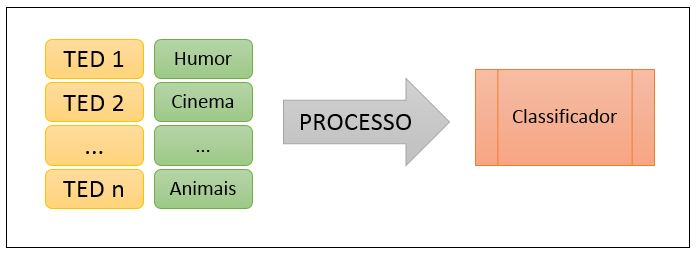
\includegraphics[scale=0.5]{modelo.JPG}
\caption{Esquema de criação do classificador}
\label{fig:modelo}
\end{figure}

\begin{figure}[h!]
\centering
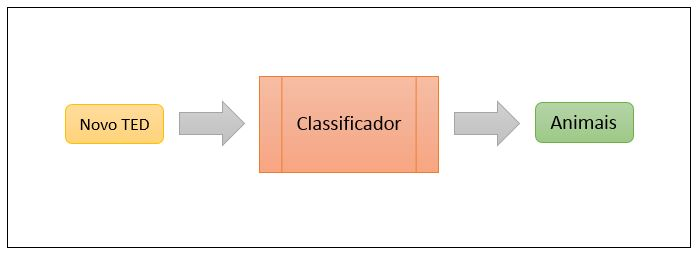
\includegraphics[scale=0.5]{classificacao.JPG}
\caption{Esquema de execução do classificador}
\label{fig:classificacao}
\end{figure}

%===============================================================
%===============================================================

\section{Proposta}

Para implementar uma solução que atenda o objetivo explicitado na seção anterior, é proposto um conjunto de ações. Essas ações foram agrupadas em etapas (Figura \ref{fig:etapas}), que serão detalhadas nas próximas seções.

\begin{figure}[h!]
\centering
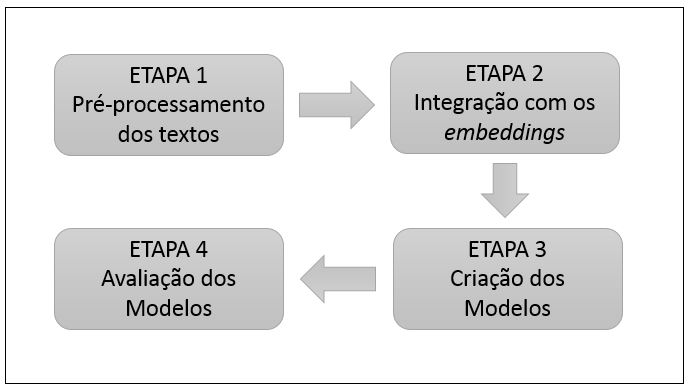
\includegraphics[scale=0.5]{etapas.JPG}
\caption{Etapas da proposta}
\label{fig:etapas}
\end{figure}

\subsection{ETAPA 1 - Pré-processamento dos textos}

O objetivo dessa seção é apresentar as atividades que foram executadas na "ETAPA 1 - Pré-processamento dos textos".\\

O primeiro passo foi fazer a leitura dos dados de entrada que foram disponibilizados em dois arquivos \textit{excel} utilizando a biblioteca Pandas \citep{pandas}. O arquivo "Transcripts.csv" armazenava as transcrições das apresentações e o arquivo "TED main.csv" armazenava os demais atributos. O primeiro processamento necessário foi a "equalização" dos dois arquivos, uma vez que o arquivo "TED main.csv" era maior, ou seja, não havia transcrições de todas as apresentações. Após isso, foi gerado um dataset com 2467 registros.\\

O segundo passo foi a eliminação dos textos que possuiam menos que 300 palavras, uma vez que seriam utilizadas 300 palavras para a criação dos embeddings. Ainda nessa etapa, foi feito o processo de tokenização, eliminação de acentos, entre outros processamentos. O resultado foi a geração de 2432 registros onde cada um armazenava as palavras de uma apresentação TED.

\subsection{ETAPA 2 - Integração com os embeddings}

O primeiro passo da ETAPA 2 foi a integração com os embeddings. Foram utilizados embeddings disponíveis na biblioteca Gensim \citep{gensim}. Dessa forma, para cada registro, que continha um conjunto maior ou igual de 300 palavras, foi feita a substituição do string da palavra pelo respectivo vetor numérico (\textit{embedding}) que representava a palavra.\\

O segundo passo foi substituir cada vetor por um valor numérico referente à média dos valores de cada vetor. Isso permitiu reduzir a dimensão da estrutura de dados utilizada que estava com 3 dimensões (uma linha por texto, uma coluna por palavra do texto, cada palavra era representada por um vetor numérico), para 2 dimensões (uma linha por texto, uma coluna por palavra do texto sendo que cada palavra era representada por um numérico).

\subsection{ETAPA 3 - Criação dos Modelos}

Após as etapas 1 e 2, foi utilizada a biblioteca Scikit-Learn \citep{scikit} para a criação de modelos de classificação. Foram gerados dois modelos: xxx e Redes Neurais (MultiLayer Perceptron). QUAL A CONFIGURAÇÃO PADRÃO DESSE MLP?

\subsection{ETAPA 4 - Avaliação dos Modelos - ACHO QUE VOU TIRAR A ETAPA 4}

Os modelos criados na ETAPA 3 foram avaliados em diferentes configurações. A seção \ref{resultados} apresenta os resultados em detalhes.

\subsection{Resumo da Proposta}

A Figura \ref{fig:fluxo} ilustra as atividades descritas nas ETAPAS 1, 2, 3 e 4.

\begin{figure}[h!]
\centering
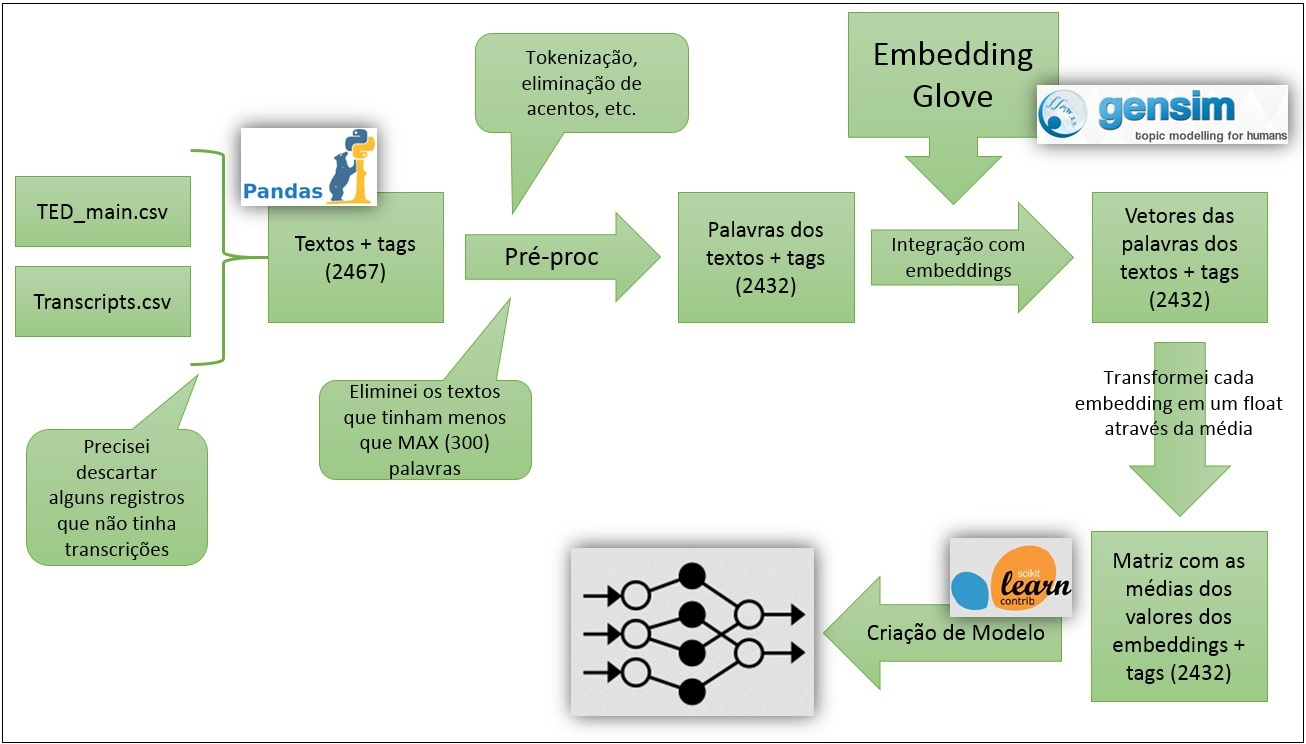
\includegraphics[scale=0.35]{fluxo2.jpg}
\caption{Detalhamento das ETAPAS 1, 2 e 3}
\label{fig:fluxo}
\end{figure}

%===============================================================
%===============================================================

\section{Análise do \textit{dataset}}

O objetivo dessa seção é fazer uma avaliação sobre o \textit{dataset} utilizado nesse trabalho \citep{datasetTED}.\\

O \textit{dataset} de apresentações TED contem xxx registros sendo que apenas yyy possuíam transcrições. Dessa forma, neste trabalho foram utilizados yyy registros.\\

Cada um dos registros possui zzz atributos: 

\begin{itemize}
\item Comentários: o número de comentários de primeiro nível feitos para a apresentação.	
\item Descrição: uma sinopse sobre o que é falado na apresentação.
\item Duração: a duração da apresentação em segundos.
\item Evento: o TED/TEDx onde a apresentação foi feita.
\item Data do filme: o timestamp Unix do filme.
\item Idiomas: o número de idiomas nos quais a apresentação está disponível.
\item Apresentador principal: o primeiro nome do apresentador.
\item Nome: o nome oficial da apresentação TED. Inclui o título e o apresentador.
\item Número de apresentadores: o número de apresentadores.
\item Data da publicação: o timestamp Unix da publicação da apresentação no site TED.com
\item Avaliações: um dicionário de strings das várias avaliações dadas à conversa (ex: inspirador, facinante, "de cair o queixo", etc.)
\item Apresentações relacionadas: uma lista de apresentações recomandadas para assistir posteriomente.
\item Ocupação do apresentador: a ocupação do principal apresentador.
\item Tags: os temas associados à apresentação.
\item Título: O título da apresentação.
\item URL: a URL da apresentação.
\item Views: O número de visualizações da apresentação.
\item Transcrição: A transcrição da apresentação em inglês.
\end{itemize}

Para a criação do classificador foram considerados os atributos "Tags" e "Transcrições". A Figura \ref{fig:qtdPorTag} apresenta os números de apresentações por "Tag".

\begin{figure}[h!]
\centering
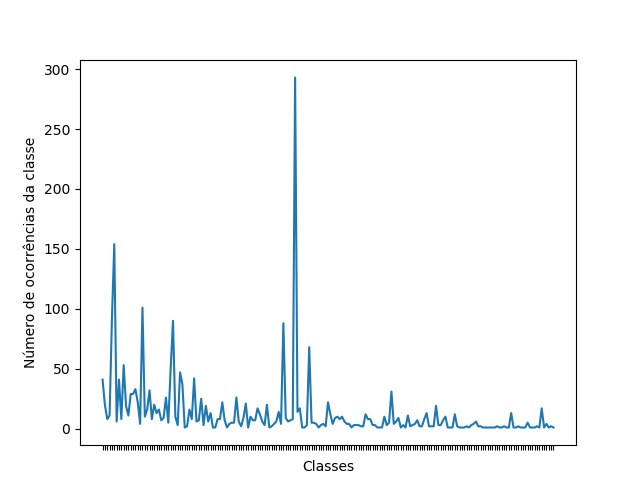
\includegraphics[scale=0.5]{qtdPorTag.JPG}
\caption{Quantidade de apresentações por tag}
\label{fig:qtdPorTag}
\end{figure}

Analisando a Figura \ref{fig:qtdPorTag} é possível perceber que a maior parte das apresentações está ... ou ... as apresentações estão espalhadas por diversos tags, sendo as maiores ... Existe um total de 193 tags, sendo que as 5 com maiores ocorrências são: TEDX: 293, BUSINESS: 154, CULTURE: 101, AFRICA: 92 e ART: 90. Sendo que 59 possuem 10 ou mais referências.

%===============================================================
%===============================================================

\section{Configurações dos Experimentos\label{configuracoes}}

O objetivo dessa seção é apresentar as configurações dos experimentos. O maior objetivo é verificar se há muita mudança nos resultados do classificador quando altero o tipo de embedding.\\

Os testes 1, 2 e 3 serão executados respectivamente com os embeddings Glove, Word2Vec e FastText. Para cada um dos testes haverá uma variação do classificador a e b, respectivamente Regressão Logística e Redes Neurais.

%===============================================================
%===============================================================

\section{Análise dos Resultados dos Experimentos\label{resultados}}

O objetivo dessa seção é apresentar os resultados dos experimentos. O código desenvolvido para a realização dos experimentos está disponível no GitHub \citep{codigo}.\\

A Tabela \ref{table:result} apresenta os resultados obtidos. Os testes utilizaram \textit{k-fold cross validation}.

\begin{table}[]
\begin{tabular}{|c|c|c|c|}
\hline
Teste & Técnica de Embedding & Regressão Logística (a) & Rede Neural (b) \\ \hline
1     & Glove                & 0,12                 & 0,08            \\ \hline
2     & Word2Vec             & 0,12                 & 0,09            \\ \hline
3     & FastText             & 0,12                 & 0,10            \\ \hline
\end{tabular}
\caption{Resultados dos Experimentos com todas as classes}
\label{table:result}
\end{table}

\begin{table}[]
\begin{tabular}{|c|c|c|c|}
\hline
Teste & Técnica de Embedding & Regressão Logística (a) & Rede Neural (b) \\ \hline
1     & Glove                & 0,16                 & 0,12            \\ \hline
2     & Word2Vec             & 0,15                 & 0,13            \\ \hline
3     & FastText             & 0,15                 & 0,12            \\ \hline
\end{tabular}
\caption{Resultados dos Experimentos com classes com mais de 10 ocorrências}
\label{table:result2}
\end{table}

Independente do modelo \textit{embedding} utilizado, o resultado foi o mesmo para o classificador Regressão Logística.\\

Utilizando o classificador Rede Neural, os resultados melhoraram com a alteração da técnica de embedding \textit{utilizada}.\\

Independente da configuração do teste, os resultados foram ruins. Um dos motivos é o grande número de classes e a existência de classes com poucas ocorrências.\\

Depois que removi as classes que tinham menos de 10 ocorrências (restaram 1962 registros e 58 classes de um total de 193), rodei novamente os testes e obtive os resultados da tabela \ref{table:result2}.\\

Os resultados apresentados na segunda tabela não foram muito diferentes dos primeiros. Acredito que a substituição dos vetores de embedding pelo valor numérico da média seja um dos fatores dos baixos resultados, uma vez que essa operação descarta parte da semântica representada pelos vetores.

%===============================================================
%===============================================================

\section{Conclusões}
%Explain the conclusions \citep{baeza1999modern} of the paper.\\

Este trabalho apresentou uma proposta de um modelo de classificação de apresentações TED com base no uso de técnicas de \textit{Word Embedding}.\\

Na realização dos experimentos foram utilizadas três técnicas de \textit{Word Embedding}: Word2Vec, GloVe e FastText.\\

Os experimentos mostraram que a variação da técnica de \textit{embedding} não influenciou muito os resultados obtidos.\\

Algumas sugestões para melhorar os resultados são: utilizar o atributo "Apresentações relacionadas" e utilizar a técnica TF-IDF para selecionar as palavras das apresentações que serão utilizadas.\\

Outra ideia possível é rever a operação de média que foi realizada sobre os vetores de \textit{embedding}.

%Outra ideia possível é utilizar um classificador multi-label, uma vez que as apresentações possuem multi classificação.

\bibliographystyle{plain}
\bibliography{references}
\end{document}
